\documentclass[tikz,border=10pt]{standalone}

\begin{document}
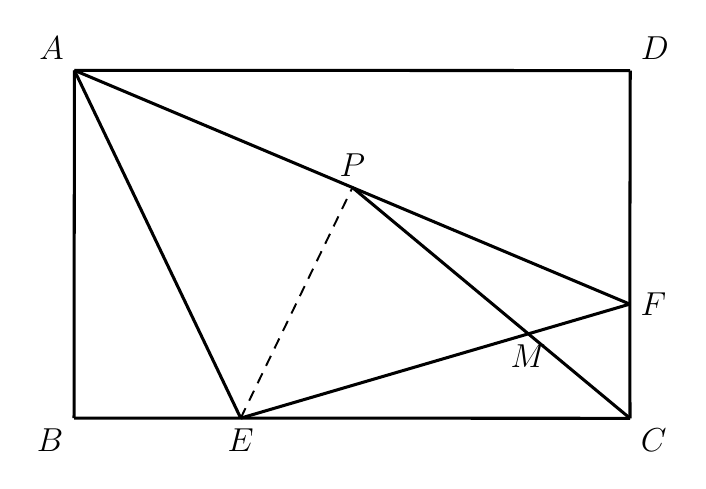
\begin{tikzpicture}[line width=1.1pt, line join=round]
\coordinate (A) at (-3.542,2.215);
\coordinate (B) at (-3.547,-2.202);
\coordinate (C) at (3.514,-2.204);
\coordinate (D) at (3.517,2.212);
\coordinate (E) at (-1.430,-2.202);
\coordinate (F) at (3.511,-0.754);
\coordinate (M) at (2.220,-1.129);
\coordinate (P) at (-0.011,0.727);

  

  
  \draw (B)--(E)--(C);   
  \draw (C)--(F)--(D);   
  \draw (D)--(A);        
  \draw (A)--(B);        

  
  \draw (A)--(E);
  \draw (E)--(F);
  \draw (A)--(P)--(F);   
  \draw (P)--(M)--(C);   

  
  \draw[dash pattern=on 4pt off 3pt, line width=0.7pt] (E)--(P);

  
  \node[above left]  at (A) {\fontsize{11.5}{13.8}\selectfont $A$};
  \node[above right] at (D) {\fontsize{11.5}{13.8}\selectfont $D$};
  \node[below left]  at (B) {\fontsize{11.5}{13.8}\selectfont $B$};
  \node[below right] at (C) {\fontsize{11.5}{13.8}\selectfont $C$};
  \node[below]       at (E) {\fontsize{11.5}{13.8}\selectfont $E$};
  \node[right]       at (F) {\fontsize{11.5}{13.8}\selectfont $F$};
  \node[above]       at (P) {\fontsize{11.5}{13.8}\selectfont $P$};
  \node[below]       at (M) {\fontsize{11.5}{13.8}\selectfont $M$};
\end{tikzpicture}
\end{document}